\subsection{Decoherence and Open Systems}
\label{subsec:decoherence}

Decoherence arises from environment interactions, modeled by the Lindblad equation:
\[
\frac{d\rho}{dt} = -\frac{i}{\hbar}[H, \rho] + \sum_k \left( L_k \rho L_k^\dagger - \frac{1}{2}\{L_k^\dagger L_k, \rho\} \right),
\]
where $L_k$ are Lindblad operators \cite{breuer2002theory}. Common noise models include:
- \textbf{Amplitude damping}: Energy loss to the environment.
- \textbf{Phase damping}: Loss of phase coherence.

\begin{figure}[h]
\centering
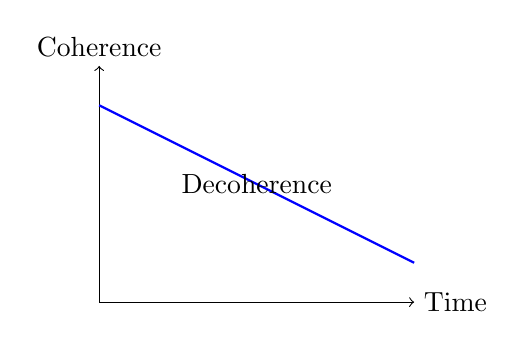
\begin{tikzpicture}
  \draw[->] (0,0) -- (4,0) node[right] {Time};
  \draw[->] (0,0) -- (0,3) node[above] {Coherence};
  \draw[thick,blue] (0,2.5) -- (4,0.5);
  \node at (2,1.5) {Decoherence};
\end{tikzpicture}
\caption{Decoherence reduces quantum state fidelity over time.}
\label{fig:decoherence}
\end{figure}

Quantum error correction codes, like the Shor code \cite{shor1995scheme}, mitigate decoherence by encoding logical qubits into multiple physical qubits.